%%%%%%%%%%%%%%%%%%%%%%%%%%%%%%%%%%%%%%%%%
% Stylish Article
% LaTeX Template
% Version 2.1 (1/10/15)
%
% This template has been downloaded from:
% http://www.LaTeXTemplates.com
%
% Original author:
% Mathias Legrand (legrand.mathias@gmail.com)
% With extensive modifications by:
% Vel (vel@latextemplates.com)
%
% Modified for General Education at Ferris State University
% by Dr. Clifton Franklund (CliftonFranklund@ferris.edu)
%
% License:
% CC BY-NC-SA 3.0 (http://creativecommons.org/licenses/by-nc-sa/3.0/)
%
%%%%%%%%%%%%%%%%%%%%%%%%%%%%%%%%%%%%%%%%%

%----------------------------------------------------------------------------------------
%	PACKAGES AND OTHER DOCUMENT CONFIGURATIONS
%----------------------------------------------------------------------------------------

\documentclass[fleqn,10pt]{SelfArx}\usepackage[]{graphicx}\usepackage[]{color}
%% maxwidth is the original width if it is less than linewidth
%% otherwise use linewidth (to make sure the graphics do not exceed the margin)
\makeatletter
\def\maxwidth{ %
  \ifdim\Gin@nat@width>\linewidth
    \linewidth
  \else
    \Gin@nat@width
  \fi
}
\makeatother

\definecolor{fgcolor}{rgb}{0.345, 0.345, 0.345}
\newcommand{\hlnum}[1]{\textcolor[rgb]{0.686,0.059,0.569}{#1}}%
\newcommand{\hlstr}[1]{\textcolor[rgb]{0.192,0.494,0.8}{#1}}%
\newcommand{\hlcom}[1]{\textcolor[rgb]{0.678,0.584,0.686}{\textit{#1}}}%
\newcommand{\hlopt}[1]{\textcolor[rgb]{0,0,0}{#1}}%
\newcommand{\hlstd}[1]{\textcolor[rgb]{0.345,0.345,0.345}{#1}}%
\newcommand{\hlkwa}[1]{\textcolor[rgb]{0.161,0.373,0.58}{\textbf{#1}}}%
\newcommand{\hlkwb}[1]{\textcolor[rgb]{0.69,0.353,0.396}{#1}}%
\newcommand{\hlkwc}[1]{\textcolor[rgb]{0.333,0.667,0.333}{#1}}%
\newcommand{\hlkwd}[1]{\textcolor[rgb]{0.737,0.353,0.396}{\textbf{#1}}}%

\usepackage{framed}
\makeatletter
\newenvironment{kframe}{%
 \def\at@end@of@kframe{}%
 \ifinner\ifhmode%
  \def\at@end@of@kframe{\end{minipage}}%
  \begin{minipage}{\columnwidth}%
 \fi\fi%
 \def\FrameCommand##1{\hskip\@totalleftmargin \hskip-\fboxsep
 \colorbox{shadecolor}{##1}\hskip-\fboxsep
     % There is no \\@totalrightmargin, so:
     \hskip-\linewidth \hskip-\@totalleftmargin \hskip\columnwidth}%
 \MakeFramed {\advance\hsize-\width
   \@totalleftmargin\z@ \linewidth\hsize
   \@setminipage}}%
 {\par\unskip\endMakeFramed%
 \at@end@of@kframe}
\makeatother

\definecolor{shadecolor}{rgb}{.97, .97, .97}
\definecolor{messagecolor}{rgb}{0, 0, 0}
\definecolor{warningcolor}{rgb}{1, 0, 1}
\definecolor{errorcolor}{rgb}{1, 0, 0}
\newenvironment{knitrout}{}{} % an empty environment to be redefined in TeX

\usepackage{alltt} % Document font size and equations flushed left
\usepackage[english]{babel}         % Specify a different language here - english by default
\usepackage{lipsum}                 % Required to insert dummy text. To be removed otherwise
\usepackage{fancyhdr}               % Required to put the logo on the top of the first page
\usepackage{float}                  % Extra help with figures and tables
\usepackage{caption}                % Helps to format captions
\captionsetup[table]{skip=3pt}      % Spacing after caption
\usepackage{enumitem}               % Tightening lists
\setlist[itemize]{itemsep=0mm}      % Tightening lists
\usepackage[style=authoryear,doi=false,isbn=false,url=false,natbib=true,backend=biber]{biblatex}
\bibliography{references}           % Point to the bibtex bibliography file
\renewbibmacro{in:}{}               % Get rid of "in:" in journal reference citations

%----------------------------------------------------------------------------------------
%	COLUMNS
%----------------------------------------------------------------------------------------

\setlength{\columnsep}{0.55cm}      % Distance between the two columns of text
\setlength{\fboxrule}{0.75pt}       % Width of the border around the abstract

%----------------------------------------------------------------------------------------
%	COLORS
%----------------------------------------------------------------------------------------

\definecolor{color1}{RGB}{0,0,0}         % Color of the article title (black)
\definecolor{color2}{RGB}{255,255,255}   % Section heading text color (white)
\definecolor{color3}{RGB}{178,34,34}     % Color of the boxes behind the abstract and headings (firebrick)

%----------------------------------------------------------------------------------------
%	HYPERLINKS
%----------------------------------------------------------------------------------------

\usepackage{hyperref}               % Required for hyperlinks
\hypersetup{hidelinks,colorlinks,breaklinks=true,urlcolor=color3,citecolor=color3,linkcolor=color1,bookmarksopen=false,pdftitle={Title},pdfauthor={Author}}

%----------------------------------------------------------------------------------------
%	NO SECTION NUMBERS
%----------------------------------------------------------------------------------------
\setcounter{secnumdepth}{0}
\setlength{\belowcaptionskip}{10pt}

%----------------------------------------------------------------------------------------
%	ARTICLE INFORMATION
%----------------------------------------------------------------------------------------

\JournalInfo{General Education Assessment}     % Report information
\Archive{Report 16(1) --- July 2016}           % Report identifier and date)

\PaperTitle{Meta-Analysis of Student Achievement on Natural Science FLO SCI1 in a 200-Level Biology Course} % Article title

\Authors{Dr. Clifton Franklund\textsuperscript{1}} % Authors
\affiliation{\textsuperscript{1}\textit{General Education Coordinator, Ferris State University}} % Author affiliation

\Keywords{Meta-Analysis --- Forest plot --- Natural Sciences --- Scientific concepts}
\newcommand{\keywordname}{Keywords} % Defines the keywords heading name

%----------------------------------------------------------------------------------------
%	ABSTRACT
%----------------------------------------------------------------------------------------

\Abstract{This report is a proof-of-concept for the proposed General Education assessment strategy at Ferris State University. Course-level student assessment data was gathered using TracDat and de-identified. The clean and tidy data set was used to generate this report using the R statistical programming language. Thirteen semesters of student performance on a lecture exam were used to evaluate student competency on Ferris Learning Outcome (FLO) SCI1. A meta-analysis of these data demonstrated that  performance was very near the criterion of success. There was substantial variation in enrollment and course performance over the time span examined The utility of reports like these to analyze, distribute, and act up General Education assessment data will be investigated using faculty focus groups in the fall of 2016.~}

%----------------------------------------------------------------------------------------
\IfFileExists{upquote.sty}{\usepackage{upquote}}{}
\begin{document}

\flushbottom % Makes all text pages the same height

\maketitle % Print the title and abstract box

\tableofcontents % Print the contents section

% Set up the first page to have the Ferris logo in the left
\fancypagestyle{firststyle}
{
	\fancyhf{}
	\fancyhead[L]{
\includegraphics[height=0.55cm]{./art/logo.png}}
}
\thispagestyle{firststyle}


%----------------------------------------------------------------------------------------
%	INITIALIZE R PARAMETERS FOR THIS DOCUMENT
%----------------------------------------------------------------------------------------








%----------------------------------------------------------------------------------------
%	ARTICLE CONTENTS
%----------------------------------------------------------------------------------------

%---------------------------
%>>>>>>>> EPIGRAPH  <<<<<<<<
%---------------------------
\begin{quote}
\begin{center}
\textit{Assessment is not a spreadsheet; \\ it's a conversation. --- Irmeli Halinen}
\end{center}
\end{quote}

%---------------------------
%>>>>>> INTRODUCTION  <<<<<<
%---------------------------
\section{Introduction} % The \section*{} command stops section numbering
%\addcontentsline{toc}{section}{Introduction} % Adds this section to the table of contents

This report is an actual analysis of real course-level assessment data from a 200-level Biology course. However, its primary purpose is to serve as a proof-of-concept for the new General Education assessment process at Ferris State University. Assessment is perhaps best viewed as a scholarly activity that is focused upon programmatic improvement. Such scholarly work should be built upon, and contribute to, the relevant professional literature \citep{Weimer2015}. To emphasize that reality, this report is formatted in the form of a journal article. This report, and ones like it, will be authored, published, and cited in future work to support the development and improvement of the General Education program at Ferris.

Many different approaches can be used to assess a General Education program; direct and indirect assessment can take place at the course, program, or institutional levels. The structure, strengths and weaknesses of each of these are highlighted elsewhere \citep{Allen2006a}. Regardless of the approach used, a quality program evaluation must possess five key attributes: utility, feasibility, propriety, accuracy, and accountability \citep{Yarbrough2011}. Both this report, and the assessment processes underlying it, are designed to satisfy these requirements.

% PROCESS FIGURE INSERTED HERE
\begin{figure*}[htb]\centering % Using \begin{figure*} makes the figure take up the entire width of the page
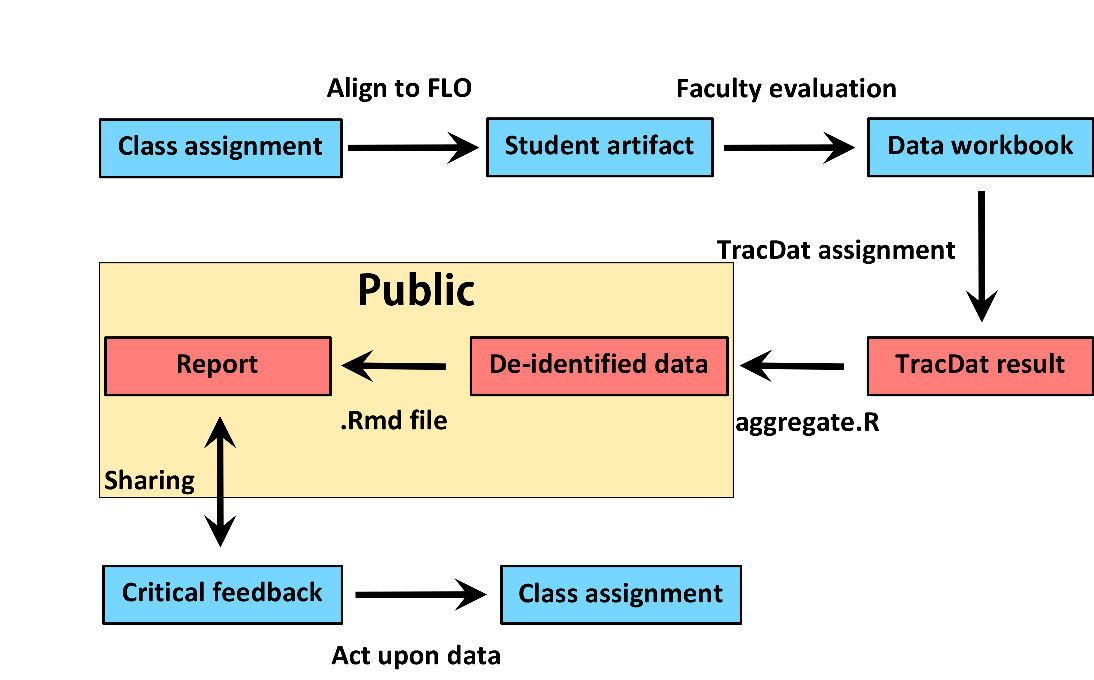
\includegraphics[width=\textwidth]{./art/process}
\protect\caption{A diagram illustrating the flow of data from initial collection to storage, access, and use. This process constitutes "closing the loop" on assessing General Education competencies. The blue boxes highlight steps with direct faculty involvement; the red boxes indicate processes carried out by the General Education Coordinator. The golden region indicates the files that are publicly available on the Open Science Framework.}
\label{fig:process}
\end{figure*}

The \textit{utility} of the assessment process is a measure of how useful it is to the relevant stakeholders. A broad sampling of our faculty are engaged in the section of assessment outcomes, collection of data, and interpretation of assessment findings. This involvement ensures that any results are viewed within an appropriate context, and increases their value for program evaluation. The automated nature of the data collection, aggregation, and analysis increases the \textit{feasibility} of this approach. Much of the reports must still be authored by the General Education Coordinator. However, having the data manipulations and analysis done automatically greatly simplifies the task. \textit{Propriety} speaks to the ethical use of the data and results. Every effort has been made to ensure that the identities of all students and faculty involved in these studies is protected. No personally identifiable information will ever be included in these results. Furthermore, the General Education assessment results exist solely for the improvement of the General Education program -- the results will \underline{never} be used for the evaluation of specific courses or instructional personnel. The \textit{accuracy} of these reports is improved by the very nature of the analysis and reporting used. Meta-analyses \citep{Borenstein2011} are used to compare groups of related assessment results. This approach can account for variation in scoring and student ability between courses and provide an a more realistic overview of student competencies. The range of meta-data collected in addition to student evaluations will permit the testing of a variety of research hypotheses. This report is also a form of reproducible research \citep{Stodden2014}. This report is computationally reproducible because the code needed to manipulate the de-identified data, perform the analyses, and create the figures are included within the no-web (.Rnw) file itself. This approach was first described as "literate programming" in the 1980's \citep{Knuth1984}. The principle advantage to this approach is that anyone (at any time) can reproduce, critique, and extend these studies without needing to track down multiple documents, graphics files, and data sets. Finally, the \textit{accountability} of reports such as this one is safeguarded by the involvement of faculty in contextualizing the results. All reports will be shared with appropriate focus groups for their input. Their comments and recommendations for future actions will be summarized and included within the discussion section of each document.

The overall process employed in this assessment strategy is illustrated in Figure \ref{fig:process} and described in the Methods. As a proof-of-concept, 13 semesters of student results from a 200-level Biology course are analyzed. A more typical analysis would be from a variety of courses (say from Biology, Chemistry, Physics, Geology, and Geography) to evaluate a specific FLO over a specific period of time.

%---------------------------
%>>>>>>>>> METHODS <<<<<<<<<
%---------------------------
\section{Methods}
%\addcontentsline{toc}{section}{Methods} % Adds this section to the table of contents

\subsection{Collection of assessment data}
Student performance on the first lecture exam in a 200-level Biology course was analyzed. The content assessed in all exams was biological diversity. However, the number and format of the questions used varied by semester. Individual student scores were collected using the new General Education Natural Sciences "scores" data workbook for 13 semesters. Student scores were automatically converted to a rubric score by the workbook using the equivalencies shown in Table \ref{tab:convert}.

% CONVERSION TABLE INSERTED HERE
\begin{table}[hbt]
\caption{Conversion of percentages to rubric scores}
\centering
\begin{tabular}{c c c}
\textbf{Percent correct} & \textbf{Rubric} & \textbf{Interpretation}   \\
\hline
 0.0 to 49.9\%   &   0   &   Unsatisfactory                                \\
50.0 to 59.9\%   &   1   &   Beginning                                     \\
60.0 to 69.9\%   &   2   &   Developing                                    \\
70.0 to 84.9\%   &   3   &   Proficient                                    \\
85.0 to 100.0\%  &   4   &   Advanced                                      \\
\end{tabular}
\label{tab:convert}
\end{table}

These workbook files contain personally identifiable information (PII) and are, therefore, subject to FERPA regulations. For this reason, they are not directly shared. Instead, they are permanently housed within the Proof\_of\_Concept folder under Core Competency: Natural Sciences in TracDat.

\subsection{De-identification of student data}
Copies of the 13 data files were downloaded from TracDat. An R aggregator script was used to read the data from these data sheets and concatenate it into one data set in a destructive process -- the downloaded copies were deleted in the process. Student names and identification numbers were redacted and each student's entry was given a unique eight-digit identifier - the Record.Key. These keys may be used for longitudinal studies in the future. The algorithm used is kept in an encrypted site and shared with \textit{no one}. The de-identified data set contains 973 student entries and is formatted as a comma-delimited text file (BIOL200Data.csv).

\subsection{Data provenance}
Data provenance refers to a system that permits tracking of the origin, movement, modification, and utilization of data sets\citep{Buneman2001}. The provenance of General Education data will be explicitly declared to facilitate the reproducibility and extensibility of these studies.

\paragraph{Location of public website files}
All files related to this report can be found online at the Open Science Framework \citep{Nosek2012}. This site contains all of the files needed to reproduce this report from the de-identified data set. The site's url is \href{https://osf.io/t6u8m/}{https://osf.io/t6u8m/}.

\paragraph{Session information}
This report was written using RStudio \citep{Rstudio} and the R statistical programming language \citep{R}. These products are free to download for PC, Macintosh, and Linux operating systems. The following information pertains to the session parameters used to generate this report. If you have trouble reproducing this report, it may be due to different session parameters. You may contact \href{mailto:CliftonFranklund@ferris.edu}{Dr. Franklund} if you need assistance.

% SESSION INFO INSERTED HERE
\begin{itemize}\raggedright
  \item R version 3.3.0 (2016-05-03), \verb|x86_64-apple-darwin13.4.0|
  \item Base packages: base, datasets, graphics, grDevices, grid,
    methods, stats, utils
  \item Other packages: car~2.1-2, dplyr~0.5.0, forestplot~1.5.1,
    Formula~1.2-1, gdata~2.17.0, ggplot2~2.1.0, Hmisc~3.17-4,
    knitr~1.13, lattice~0.20-33, magrittr~1.5, mice~2.25,
    modeest~2.1, moments~0.14, papeR~1.0-1, Rcpp~0.12.6,
    survival~2.39-5, weights~0.85, xtable~1.8-2
  \item Loaded via a namespace (and not attached):
    acepack~1.3-3.3, assertthat~0.1, chron~2.3-47, cluster~2.0.4,
    colorspace~1.2-6, data.table~1.9.6, DBI~0.4-1, evaluate~0.9,
    foreign~0.8-66, formatR~1.4, gmodels~2.16.2, gridExtra~2.2.1,
    gtable~0.2.0, gtools~3.5.0, latticeExtra~0.6-28, lme4~1.1-12,
    MASS~7.3-45, Matrix~1.2-6, MatrixModels~0.4-1, mgcv~1.8-13,
    minqa~1.2.4, munsell~0.4.3, nlme~3.1-128, nloptr~1.0.4,
    nnet~7.3-12, parallel~3.3.0, pbkrtest~0.4-6, plyr~1.8.4,
    quantreg~5.26, R6~2.1.2, RColorBrewer~1.1-2, rpart~4.1-10,
    scales~0.4.0, SparseM~1.7, splines~3.3.0, stringi~1.1.1,
    stringr~1.0.0, tibble~1.1, tools~3.3.0
\end{itemize}


\paragraph{Processing instructions}
This project produced a computationally reproducible assessment report (this document). Anyone wishing to recreate this report from the source document will need to install the following on their computer:
\begin{enumerate}
\item \href{https://www.r-project.org}{An installation of the R programming language}
\item \href{https://www.rstudio.com/products/rstudio/download3/}{ An installation of the RStudio IDE}
\item \href{https://www.latex-project.org/get/}{An installation of \LaTeX}
\end{enumerate}

The necessary source files include the de-identified data set (BIOL200Data.csv), no-web code file (Gen\_Ed\_Report\_16-01.Rnw), bibtex reference file (references.bib), and custom art file in the /art folder.

To process the files, you must first open the .Rnw file in RStudio. Click on the "Compile PDF" button in the menu bar. The resulting tex file (Gen\_Ed\_Report\_16-01.tex) must be further processed to create the citations and internal links. This is done by running PDFLaTeX on the .tex file, followed by biber, and then PDFLaTeX twice more. This report will be the resulting pdf file.

\paragraph{Citation of this work}
All of the de-identified data, analysis code, and documentation that constitute this report project may be freely used, modified, and shared. The code file, Gen\_Ed\_Report\_16-01.Rnw, was adapted from that of Matias Legrand. Like the original file, it is released under the Creative Commons \href{http://creativecommons.org/licenses/by-nc-sa/3.0/}{CC BY-NC-SA 3.0} license. The de-identified data set, BIOL200Data.csv, is released under the Creative Commons \href{https://creativecommons.org/publicdomain/zero/1.0/}{CC0 license}. All documentation, including README.md, Codebook.md, and this report, are released under the Creative Commons \href{https://creativecommons.org/licenses/by/4.0/}{CC-BY} licence. Any questions, comments, or suggestions may be sent to \href{mailto:CliftonFranklund@ferris.edu}{Dr. Franklund}.


%---------------------------
%>>>>>>>>> RESULTS <<<<<<<<<
%---------------------------
\section{Results}
This document itself is the primary result of the project. It will be shared with members of the General Education Committee, Academic Senate, and the Department of Biological Sciences at Ferris State University. Their comments and suggestions will be included in the Discussion.

% T-test calculation


\subsection{Summary statistics}
A total of 973 student performances on exam 1 were collected over 13 semesters of instruction. Student scores were converted to rubric scores as described above. The overall average rubric score for all students and semesters was 2.54. The mode and median scores were 3 and 3, respectively. The average was not statistically different from the threshold score for competence (2.6) as evaluated with a one-value, two-tailed t-test (t=\ensuremath{-1.71}, df=972, p=0.087). The effect size for the difference between the average and the threshold was tiny (d=\ensuremath{-0.05}). We can infer from this that the overall average rubric score is not practically different than the threshold score.
% HISTOGRAM FIGURE INSERTED HERE
\begin{figure}[h]\centering

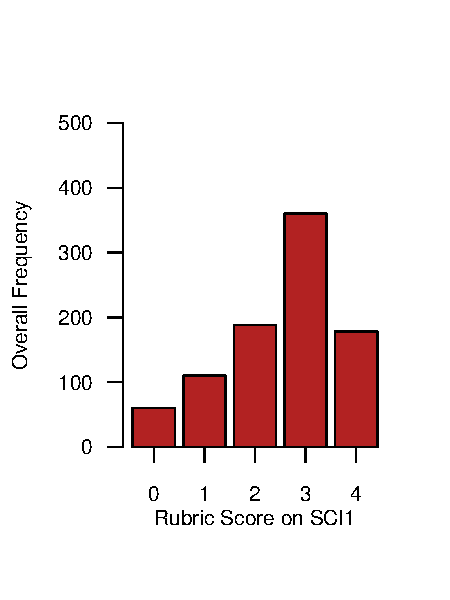
\includegraphics[width=\columnwidth,viewport = 0 20 216 240]{./figure/histogram}
\protect\caption{A histogram of the distribution of individual rubric score frequencies over all thirteen semesters.}
\label{fig:histogram}
\end{figure}

The distribution of all rubric scores is shown in Figure \ref{fig:histogram}. This distribution exhibited a moderate negative skew (skew = \ensuremath{-0.62}). This result may simply indicate that the teaching, materials, and student learning are all functioning well when the scores are viewed in aggregate. A total of 583 students (59.9\%) met or exceeded the competence threshold over the semesters investigated.

The distribution of rubric scores by semester is shown in Figure \ref{fig:barplot}. There are rather obvious differences in both the distribution of rubric scores and class sizes between semesters. A one-way ANOVA was used to compare the rubric scores by semester (Table \ref{tab:anova}). Unsurprisingly, there were statistically significant differences between semester scores. Semester of instruction, however, explained a relatively small amount of the overall variance ($\eta^2$ = 0.11).

% BARPLOT FIGURE INSERTED HERE
\begin{figure}[h]\centering

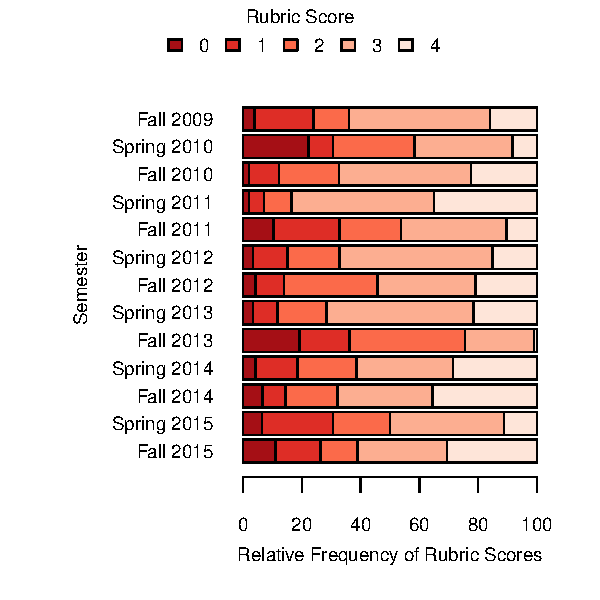
\includegraphics[width=\columnwidth,viewport = 30 0 288 288]{./figure/barplot}
\protect\caption{A barplot showing the distribution of rubric scores broken down by semester.}
\label{fig:barplot}
\end{figure}

% ANOVA TABLE INSERTED HERE
\begin{center}
% latex table generated in R 3.3.0 by xtable 1.8-2 package
% Sun Aug 28 15:11:30 2016
\begin{table}[ht]
\centering
\caption{One-way ANOVA analysis of scores by semester} 
\label{tab:anova}
\begin{tabular}{lrrrrr}
  \hline
 & Df & Sum Sq & Mean Sq & F value & Pr($>$F) \\ 
  \hline
Semester & 12 & 142.74 & 11.89 & 9.85 & 0.0000 \\ 
  Residuals & 960 & 1159.22 & 1.21 &  &  \\ 
   \hline
\end{tabular}
\end{table}

\end{center}

\subsection{Meta-analysis}
Meta-analysis of the student performance was performed using R \citep{TQMP11-1-37}. This analysis resulted in a weighted average of rubric scores. This value was calculated using formula \ref{eq:weightX}. The value X\textsubscript{i} average rubric scores for the semesters, while P\textsubscript{i} is the weighting factor (student enrollment).

\begin{equation}
\bar{X}_w = \frac{\sum X_i P_i}{\sum P_i}
\label{eq:weightX}
\end{equation}

The confidence interval for the weighted mean was calculated using the weighted variance. However, the weighted variance is actually not simple to calculate. Several different methods have been compared to bootstrapping \citep{Gatz1995a}. The most accurate method was initially described by Cochran \citep{Cochran1977} and that one was used in this study. The calculation to obtain the weighted variance is shown in formula \ref{eq:weightV}.

\begin{equation}
\begin{split}
(SEM_w)^2 = \frac{n}{(n-1)(\sum P_i)^2}\big[ \sum(P_i X_i - \bar{P}\bar{X}_w)^2 \\
- 2\bar{X}_w \sum(P_i - \bar{P})(P_i X_ i - \bar{P} \bar{X}_w) + \bar{X}_w^2 \sum(P_i - \bar{P})^2 \big]
\label{eq:weightV}
\end{split}
\end{equation}


% INSERT FOREST PLOT HERE
\begin{figure*}[htb]\centering % Using \begin{figure*} makes the figure take up the entire width of the page

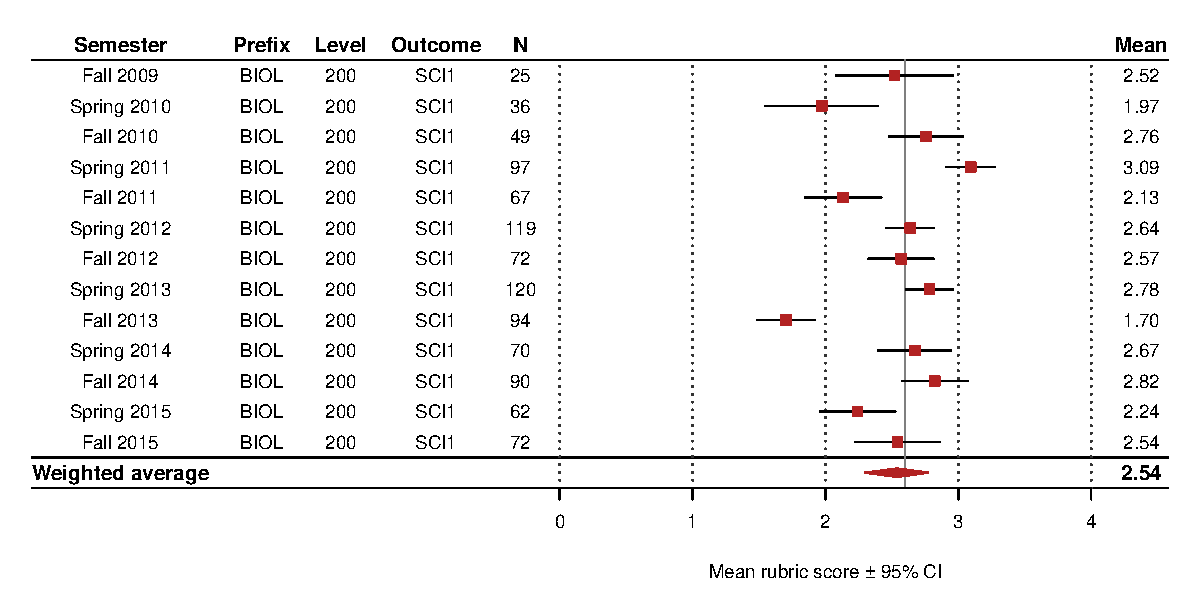
\includegraphics[width=\textwidth]{./figure/forest}
\protect\caption{A forest plot of the average scores for each semester with a weighted mean estimate for the entire period investigated. Error bars indicate the 95\% confidence intervals.}
\label{fig:forest}
\end{figure*}

% CALCULATE WEIGHTED T-TEST


A forest plot of the meta-analysis is shown in Figure \ref{fig:forest}. In this representation, each semester is illustrated as a separate line. The mean and 95\% confidence intervals for each semester are plotted in the right panel and their associated meta-data are given in the table to the left. The weighted average of all the data is plotted at the bottom of the figure. The width of the diamond indicates the 95\% confidence interval.

The rubric scale can be conceptually divided into five areas as shown in Table \ref{tab:regions}. Of the 13 semesters, 6 fell in the proficient range, 6 fell in the developing range, and 1 fell in the beginning range. The weighted mean score, 2.54, was not significantly different from the threshold of competence as judged by a weighted, one-factor, two-tailed t-test (t=\ensuremath{-0.57}, df=12, p=0.58). We can conclude that the weighted average score is practically equivalent to the competency threshold score.

\begin{table}[hbt]
\caption{Interpretation of average rubric scores}
\centering
\begin{tabular}{c c}
\textbf{Average score} & \textbf{Interpretation}   \\
\hline
0.00 to 0.99   &   Unsatisfactory                                \\
1.00 to 1.79   &   Beginning                                     \\
1.80 to 2.59   &   Developing                                    \\
2.60 to 3.39   &   Proficient                                    \\
3.40 to 4.00   &   Advanced                                      \\
\end{tabular}
\label{tab:regions}
\end{table}


%---------------------------
%>>>>>>> DISCUSSION  <<<<<<<
%---------------------------
\section{Discussion}
%\addcontentsline{toc}{section}{Results and Discussion} % Adds this section to the table of contents

A novel approach for the collection, aggregation, analysis, and reporting of General Education assessment data has been developed. Computationally reproducible reports can easily be generated and distributed to improve the program over time. A meta-analysis of data collected from a 200-level Biology course was used as a proof-of-concept.

Over a span of 13 semesters, 46.2\% of courses had mean scores considered to be proficient. Of all students in all semesters, 59.9\% met or exceeded the competence threshold. From these data it is inferred that the students meet (just barely) the threshold of competence.

\subsection{Faculty feedback}
This report will be distributed to members of the General Education Committee, Academic Senate, and the Department of Biological Sciences.  These individuals will be asked to provide their comments, suggestions, and concerns about this report and the processes involved in its creation. What thoughts do you have about:

\begin{itemize}[noitemsep]
\item The data provenance plan?
\item The format of this report?
\item The content of this report?
\item The utility of the meta-analysis?
\item The public release of assessment results?
\item Any other topics you can think of?
\end{itemize}

\subsection{Plan of action}
After analyzing the data and considering the comments provided in the faculty feedback, the relevant General Education sub-committee members will make one or more recommendations for future work. Some of the possible actions could include:
\begin{itemize}[noitemsep] % [noitemsep] removes whitespace between the items for a compact look
\item No modifications -- continue to gather data
\item Convene a training session to get better inter-course reliability
\item Suggest modifications to the types of assignments that are used
\item Suggest modifications to which data workbooks are used
\item Suggest that instructors consider modifying the scope or sequence of instruction
\item Modify the learning outcomes themselves
\item Modify the competency as a whole
\end{itemize}

%---------------------------
%>>>>> ACKNOWLEDGMENTS <<<<<
%---------------------------
\phantomsection
\section*{Acknowledgments} % The \section*{} command stops section numbering
\addcontentsline{toc}{section}{Acknowledgments} % Adds this section to the table of contents

This report was based off of a \LaTeX{} template created by Mathias Legrand. The original file can be accessed at: \\
\href{http://www.latextemplates.com/template/stylish-article}{http://www.latextemplates.com/template/stylish-article}. \\
The valuable contributions made by the members of the General Education Committee, Academic Senate, and Department of Biological Sciences are also greatly appreciated.

%---------------------------
%>>>>>>> REFERENCES  <<<<<<<
%---------------------------
\phantomsection
\printbibliography[title={References},heading=bibintoc]


%----------------------------------------------------------------------------------------

\end{document}
